%%%%%%%%%%%%%% IROS %%%%%%%%%%%%%%%%%%
%\documentclass[letter, 10pt, conference]{ieeeconf}      % Use this line for a4 paper
%
%\IEEEoverridecommandlockouts                              % This command is only needed if 
%                                                          % you want to use the \thanks command
%
%\overrideIEEEmargins                                      % Needed to meet printer requirements.

%%%%%%%%%%%%% RSS %%%%%%%%%%%%%%%%%%%%
\documentclass[conference]{IEEEtran}
\usepackage{times}
\usepackage[numbers]{natbib}
\usepackage{multicol}
\usepackage[bookmarks=true]{hyperref}

\newcommand{\reals}{\mathbb{R}}

% LTL
\newcommand{\true}{\emph{true}}
\newcommand{\false}{\emph{false}}
\newcommand{\X}{\textbf{\textsc{X}}}
\newcommand{\U}{\textbf{\textsc{U}}}
\newcommand{\G}{\textbf{\textsc{G}}}
\newcommand{\F}{\textbf{\textsc{F}}}

% LDBA
\newcommand{\ba}{\mathcal{A}}
\newcommand{\lang}{\mathcal{L}}
\newcommand{\alphabet}{2^\ap}
\newcommand{\lts}{\mathcal T}

% Product
\newcommand{\product}{\mathcal{P}}



\newcommand{\environment}{\mathcal{X}}
\newcommand{\initpoint}{x_0}
\newcommand{\obstacle}{\mathcal{O}}
\newcommand{\labelling}{{L}}
\newcommand{\ap}{\Sigma}
\newcommand{\spec}{\Phi}
\newcommand{\leveldomain}{\mathcal{D}}
\newcommand{\transitions}{\Delta}
\newcommand{\sampledpoint}{x_{s}}
\newcommand{\neighbour}{x_{near}}
\newcommand{\samplingthreshold}{\theta_s}
\newcommand{\learnthreshold}{\theta_l}
\newcommand{\sensingradius}{r_s}
\newcommand{\robotposition}{x_R}
\newcommand{\nextposition}{x_{next}}
\newcommand{\freespace}{\environment_{\text{free}}}
\newcommand{\traj}{\sigma}


% ALGORITHMS
\newcommand{\explored}{explored}
\newcommand{\states}{S}
\newcommand{\initstate}{s_0}
\newcommand{\bias}{bias}
\newcommand{\biassource}{source}
\newcommand{\biasdest}{dest}
\newcommand{\sampled}{sampled}
\newcommand{\abstraction}{abstraction}
\newcommand{\similar}{t_{sim}}
\newcommand{\reachable}{reached}
\newcommand{\final}{final}
\newcommand{\moverobot}{moveRobot}
\newcommand{\radius}{r}
\newcommand{\modes}{\mathbb{M}}
\newcommand{\modemap}{\mathcal{M}}
\newcommand{\DOC}{\mathit{DoC}}

\let\proof\relax
\let\endproof\relax
\usepackage{amsthm}
\newtheorem{theorem}{Theorem}
\newtheorem{definition}{Definition}
\newtheorem{problem}{Problem}
\newtheorem{lemma}{Lemma}
\theoremstyle{remark}
\newtheorem{remark}{Remark}
\newtheorem{example}{Example}


\newcommand{\todo}[1]{{\color{red}#1}}


\newcommand{\sep}{Explore, then plan}
\newcommand{\tog}{Simultaneous}
\newcommand{\bia}{Simult.\ biased}
% The following packages can be found on http:\\www.ctan.org
%\usepackage{graphics} % for pdf, bitmapped graphics files
%\usepackage{epsfig} % for postscript graphics files
%\usepackage{mathptmx} % assumes new font selection scheme installed
%\usepackage{times} % assumes new font selection scheme installed


\usepackage{amsmath} % assumes amsmath package installed
\usepackage{amssymb}  % assumes amsmath package installed


\usepackage[english]{babel}
%\usepackage{algorithmicx,algorithm}
%\usepackage[noend]{algpseudocode}
\usepackage[ruled,vlined,linesnumbered]{algorithm2e}
\usepackage{multirow}
\usepackage{soul}
\usepackage{booktabs}
\usepackage[caption=false]{subfig}

\usepackage{tikz}
\usetikzlibrary{arrows,automata}
\usetikzlibrary{positioning}


\tikzset{
    state/.style={
           rectangle,
        %   rounded corners,
           draw=black, very thick,
           minimum height=2em,
           inner sep=2pt,
           text centered,
           },
}


% RSS: remove \LARGE \bf
\title{
Semantic Abstraction-Guided Motion Planning \\ for scLTL Missions in Unknown Environments
%LTL Motion Planning Guided by Semantic Abstractions
}

% RSS: 
\author{Author Names Omitted for Anonymous Review.}
% IROS:
%\author{Kush Grover$^{1}$ \and Fernando S. Barbosa$^{2}$ \and Jana Tumova$^2$ \and Jan K\v ret\'insk\'y$^1$% <-this % stops a space
% \thanks{*This work was not supported by any organization}% <-this % stops a space
%\thanks{$^{1}$ Technical University of Munich, Germany. 
%        {\tt\small \{grover, jan.kretinsky\}@in.tum.de}}%
%\thanks{$^{2}$KTH Royal Institute of Technology, Stockholm, Sweden.
%        {\tt\small \{fdsb, tumova\}@kth.se}}%
%}

\begin{document}


% \theoremstyle{theorem}
% \theoremstyle{definition}
% \theoremstyle{problem}


\maketitle

% RSS: remove the following 2 lines
%\thispagestyle{empty}
%\pagestyle{empty}


%%%%%%%%%%%%%%%%%%%%%%%%%%%%%%%%%%%%%%%%%%%%%%%%%%%%%%%%%%%%%%%%%%%%%%%%%%%%%%%%
\begin{abstract}
Complex mission specifications can be often specified through temporal logics, such as Linear Temporal Logic and its syntactically co-safe fragment, scLTL. Finding trajectories that satisfy such specifications becomes hard if the robot is to fulfil the mission in an initially unknown environment, where neither locations of  regions or objects of interest in the environment nor the obstacle space are known a priori. We propose an algorithm that, while exploring the environment, learns important semantic dependencies in the form of a semantic abstraction, and uses it to bias the growth of an RRG graph towards faster mission completion. Our approach leads to finding trajectories that are much shorter than those found by the sequential approach, which first explores and then plans. Simulations comparing our solution to the sequential approach, carried out in 100 randomized office-like environments, show more than 50\% reduction in the trajectory length.
\end{abstract}

% RSS:
\IEEEpeerreviewmaketitle

%%%%%%%%%%%%%%%%%%%%%%%%%%%%%%%%%%%%%%%%%%%%%%%%%%%%%%%%%%%%%%%%%%%%%%%%%%%%%%%%

\section{Introduction}

%Sampling-based motion planning is a well-developed area with plenty of applications \todo{cite some survey} and techniques available, for instance, RRT, RRG \todo{list and cite relevant stuff}.

Motion planning with Linear Temporal Logic (LTL) mission specifications aims for consideration of richer objectives than the traditional A-to-B motion planning. Examples of such objectives include periodic surveillance, request-response, or sequencing. Successful approaches to the problem range from using various cell decomposition techniques, to creating roadmaps abstracting the environment and to sampling-based motion planning. Motion planning with LTL missions is, however, much more challenging in \emph{a priori} unknown environments: efficient treatment of LTL specifications may require exploiting semantic and spatio-temporal dependencies between features of the environment, which are typically unknown beforehand. As an example, consider that we would like a robot to check all waste bins in all offices in an office environment. When finding the first bin, the robot may realize it was next to a desk. While looking for the bin in the next office, it is most natural that the robot starts exploring again next to the desk. At the same time, due to the potential complexity of the environment, it is not desirable to stick fully to all of the observed semantic and spatio-temporal correlations as not all of them are relevant for the specification satisfaction.

%However, techniques tailored or even just applicable to the setting with rich specifications, such as formulae of Linear Temporal Logic (LTL) are scarce \todo{I'm not sure about it (for LTL motion planning there is probably plenty, but sampling-based? if still plenty then we'd restrict already here to partially known labellings); cites}.
%The difficulties arising due to rich logical specifications are twofold.
%Firstly, it is hard to find a satisfying path by a simple random exploration of the state space.
%Indeed, a very particular (and thus rare order) of events may be required, followed by an infinite repetition of its (possibly non-trivial) modifications as the plan does not depend on the current state only but also on the history.
%Secondly, efficient treatment of specifications in temporal logic may require exploiting semantic and spatio-temporal dependencies between atomic propositions, which are typically unknown.
%Moreover, even if there is some domain knowledge or learnt experience, it is hard to reflect.

%\begin{example*}

% As an example, consider an LTL goal specification $\F(\mathit{living\_room}\wedge\F \mathit{kitchen}) \wedge \F\mathit{kitchen}$ expressing that   

% encoding a sequence of, e.g., collecting A and then B (B's before A do not count), and a property $\psi=\F c$. % $\psi=\F(d\wedge \F e)$ for switching off the collector and then switching off entirely.
% For the specification $\varphi\wedge\psi$, it might seem sensible to take $c$ if the opportunity occurs, so that we make progress w.r.t.~$\psi$.
% However, we might experimentally observe that we see no $a$'s and $b$'s occur after $c$ (for instance since $c$ denotes switching off the collector), while otherwise $b$'s are frequent if no $c$ is taken.
% As a consequence of this learnt conjecture, we might rather counter-intuitively postpone any progress with $c$, wait for an $a$, then take the abundant $b$ and only afterwards take $c$.
% While such a plan might be still discovered by random trials, if the sequences are longer then we need this kind of learning and reasoning to get reasonably high chance thereof.
% %\end{example}

In this paper, we focus on sampling-based motion planning with missions specified with the syntactically co-safe fragment of LTL (scLTL), and with the robot deployed in \emph{a priori} unknown environments.
%we address both difficulties in the setting of sampling-based motion planning with LTL specifications where, moreover, the atomic-proposition labelling may not be completely known for the whole state space upfront, but only for some sensing radius.
The key idea of our approach is, on the conceptual level, to make the sampling \emph{guided} by a semantic abstraction of the system and by the specification. 
%moreover, \emph{in connection to the system}.
%In our example, the property might guide us to take $c$ since we are waiting for it, but the achieved knowledge of the system w.r.t.\ this property dissuades us from doing so.
The overview of our algorithm is depicted in Fig.~\ref{fig:guide}. We extend the RRG algorithm with learning and biasing; we iteratively learn a semantic abstraction of the system from the gradually growing RRG graph and compose it with an automaton representation of the specification into a so-called product. The product is used to bias sampling in RRG, i.e. to exploit the semantic and spatio-temporal dependencies of features in the environment as well as their relation to satisfying the desired specification.

%On the technical level, we \texttt{learn} a %\emph{semantic abstraction of the system}  and use its \emph{product with the property automaton} to \texttt{bias} further sampling.
%The states of the semantic abstraction reflect (only) the logical validity of \todo{atomic propositions}; its transitions are learnt from the samples, which are anyway generated in the RRG-based planning.



% \begin{figure}
%     \centering
%     \includegraphics[scale=0.6]{scheme}
%     \caption{Guidance scheme \todo{think of a good way to draw this}}
%     \label{fig:scheme}
% \end{figure}
\begin{figure}
    \centering
    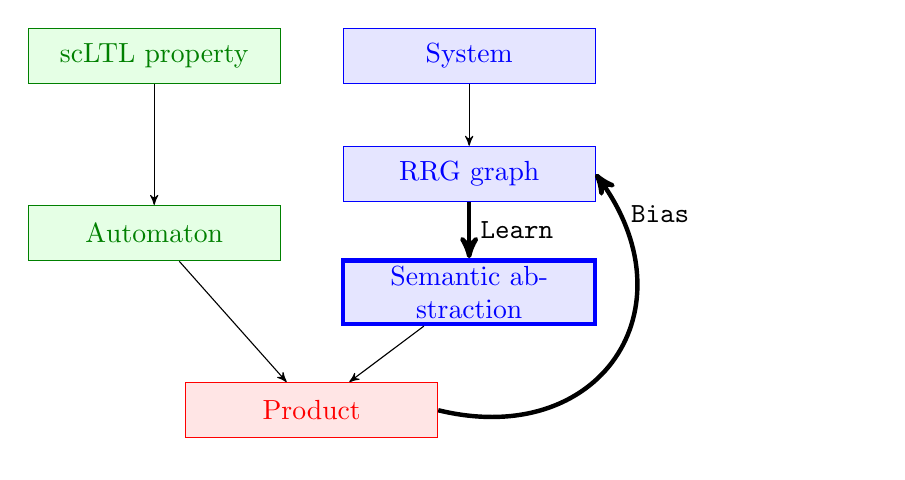
\begin{tikzpicture}[->,>=stealth', minimum width = 32mm,text width = 30mm]
        \node[state=initial, color = blue, anchor=center, fill = blue!10!white,thin] (A) {System};
        \node[state, color = blue, below of = A, fill = blue!10!white, node distance =1.5cm,thin] (B) {RRG graph};
        \node[state, color = blue, below of = B, fill = blue!10!white, node distance =1.5cm,ultra thick] (C) {Semantic abstraction};
        \node[state, color = red, below of = C, fill = red!10!white, xshift = -2cm, node distance =1.5cm,thin] (D) {Product};
        \node[state, color = green!50!black, left of = A, fill = green!10!white, node distance =4cm,thin] (E) {scLTL property};
        \node[state, color = green!50!black, below of = E, fill = green!10!white, node distance =2.25cm,thin] (F) {Automaton};
        
        \path (A) edge[] (B)
        (B) edge[ultra thick] node[right,pos=0.5]{\texttt{Learn}} (C)
        (C) edge (D)
        (E) edge (F)
        (F) edge (D)
        (D.east) edge[bend right=70,looseness=1.5, ultra thick] node[right,pos=0.9]{\texttt{Bias}} (B.east)
        %guidance $\rightarrow$ better paths and learning w.r.t. property
        ;
    \end{tikzpicture}
    \caption{Scheme of our model-checking-inspired approach with novel elements drawn thickly. }
    \label{fig:guide}
\end{figure}

%The specification is thus exploited twice to improve the guidance: (1) We reflect the property itself. (2) We can build the product and reflect the particularities of the (unknown) system \emph{behaviour with respect to the property}.

Compared to the naive two-step approach, which first explores the environment and then plans a trajectory that satisfies the mission, our approach (i) performs both tasks at once and, moreover, (ii) allows mutual exchange of information between the two tasks. 
We show that these two improvements shorten the length of the executed path significantly.
We achieve this while maintaining similar computation time, which will, in reality, be negligible as the robot can execute the algorithm in real-time while navigating in the environment.
Our contribution can be summarized as follows:
\begin{itemize}
    \item We propose a method to learn a semantic abstraction of the system, suitable for planning with scLTL missions. 
    \item We exploit the learned semantic abstraction and, together with consideration of the specification, we bias the growth of the RRG graph towards promising regions (in terms of making progress towards the specification satisfaction).
    \item We experimentally show that the loop between sampling and learning leads to better planning in terms of shorter trajectories when compared to the naive two-step approach. The results indicate more than $50\%$ savings.
    %, and (2) more goal-oriented and thus more explainable plans.
\end{itemize}



The paper is organized as follows. Sec.~\ref{sec:related} introduces relevant related work, and Sec.~\ref{sec:prel} describes preliminary tools needed for the remainder of the paper. The problem is formally defined in Sec.~\ref{sec:prob}, which is followed by the proposed solution and analysis in Sec.~\ref{sec:sol}. Lastly, a case study is presented in Sec.~\ref{sec:cases}, with conclusions and future work in Sec.~\ref{sec:conclusion}.


%\todo{Mention somewhere that partitioning according APs is a very simple semantic abstraction -- tells us only where interesting properties are and how they neighbor with each other}

\subsection{Related Work} \label{sec:related}
One of the first works to propose the use of a sampling-based motion planning algorithm to find a trajectory that satisfies a temporal logic specification is \cite{karaman2009sampling}. In that work, the authors propose the Rapidly-exploring Random Graph (RRG) as an alternative to the Rapidly-exploring Random Tree (RRT) to finding cyclic trajectories that satisfy a deterministic $\mu$-calculus specification. Another approach is presented in \cite{bhatia2010sampling}, but this time for the syntactically co-safe fragment of Linear Temporal Logic (scLTL). Following these, \citet{vasile2013sampling} propose improvements to \cite{karaman2009sampling}, more specifically for dealing with full LTL and for improving scalability. None of these works, however, deals with partially-known environments, nor do they attempt to speed up the search by learning characteristics of the environment.

More recently, \citet{kantaros2018sampling} described an approach for multi-robot systems under global temporal tasks. Instead of using an RRG, the authors propose a two-step approach using RRT$^\star$. The first step constructs a tree until an accepting state of the automaton capturing the evolution of the LTL formula is reached. The second step then grows another tree rooted at this accepting state, and attempts to find a cyclic (infinite) path that satisfies the LTL specification. The same authors then introduce in \cite{kantaros2020stylus} sampling bias guided by the automaton capturing the LTL, something that \cite{luo2019abstraction} also proposes in a similar fashion. Lastly, besides proposing a heuristic to guide the search, \cite{tajvar2020safe} integrates feedback control laws to guarantee feasibility of plans by robots with complex, possibly non-holonomic, dynamics. Although these works propose ways of improving the time taken to find a plan, they all rely on having details of the environment a priori.

To the best of our knowledge, the two papers that are mostly related to ours are \cite{kantaros2020reactive} and \cite{ayala2013temporal}. The former proposes a reactive sampling-based algorithm for path planning in unknown environments under scLTL specifications. However, differently from what we propose, only the obstacle space is initially unknown to \cite{kantaros2020reactive}, i.e. the locations of the regions of interest, therefore the labeling function, are {known} a priori. On the other hand, \citet{ayala2013temporal} considers completely unknown environments, including the labeling function. However, the authors propose an approach over a discretized partitioning of the environment, performing frontier exploration \cite{yamauchi1997frontier} until a path that satisfies the scLTL specification is found. We merge benefits of both approaches by proposing a sampling-based approach on completely unknown environments; furthermore, we propose a way of learning relations between labels, together with exploiting them for guiding the path search.


When it comes to robotic deployment in unknown environments, a crucial initial step might be to efficiently create a map in an exploratory manner. A seminal work on exploration is by \citet{yamauchi1997frontier}, in which the author proposes the method coined \emph{frontier exploration}. Since then, several other approaches have been proposed. Among them is the Receding Horizon Next-Best-View Planner \cite{bircher2016receding} and the Autonomous Exploration Planner \cite{selin2019efficient}, both building upon RRT$^\star$. These works, however, do not focus on capturing various dependencies and relations in the environment. In  contrast, in a probabilistic approach proposed by \citet{aydemir2013active}, a robot uses common-sense knowledge about the relation between objects and semantic room categories. Here, the focus is however on search for objects and not satisfaction of complex LTL goals. 
%These approaches can be used as fallback cases in our algorithm; i.e. when our approach still does not have enough information to bias the growth of the RRG graph, it need to take a step towards exploring the space in a promising direction.

\section{Preliminaries}\label{sec:prel}

Let $\reals$ denote the set of real numbers and $\reals^n$ the $n$-dimensional Euclidean space. 
We use $\ap$  for the finite set of atomic propositions.
For a set $X$, $2^X$ denotes its power set.
%and $X^\omega$ denotes its countably infinite product $(X\times X\times X\dots)$, also called the set of infinite words over $X$. 
A word over an alphabet $Y$ is a sequence of elements of $Y$.
The exclusive-or operation is denoted by $\oplus$, and the disjoint union of sets by $\uplus$.

Consider a robot deployed in an \emph{environment} $\environment \subset \reals^n$ and let $\initpoint \in \environment$ be its initial state. Let $\{\obstacle_1, \obstacle_2, \dots \obstacle_k\}$ be the set of obstacles such that $\obstacle_i\subset \environment$ for all $i \in [1,k]$, and $\freespace = \environment \setminus \bigcup_{i=1}^{k} \obstacle_i$ denotes the obstacle-free space.
A trajectory in the environment $\environment$ is defined by a continuous function $\traj:~[0,1] \to \environment$. 
A trajectory is collision-free if $\traj(t) \in \freespace$, $\forall t \in [0,1]$. 
Regions of the environment $\environment$ are labelled with atomic propositions $\ap$ according to a labelling function $\labelling : \environment \rightarrow 2^{\ap}$, which maps each state in the state-space to a set of atomic propositions that hold true there.

A map of the environment $\environment$ is a partitioning into a finite number of cells of equal size with a predefined precision, which can be labeled as \emph{free}, meaning that the cell lies in $\freespace$, \emph{occupied}, if any point within the cell lies inside the obstacle space (corresponding to an over-approximation of the obstacle set), or \emph{unmapped}, that highlights the cell has not been seen by the robot so far. Every cell is initialised as \emph{unmapped}, and is updated whenever it lies in the line-of-sight of the robot. A cell is called a \emph{frontier} cell if it is marked as \emph{free} and has a neighbouring cell marked as \emph{unmapped}. A \emph{map frontier} is a connected group of frontier cells, and its size is its cardinality.
This is a common approach among the 3D-exploration community, so we refer to papers such as \cite{yamauchi1997frontier,bircher2016receding} for more details.

\subsection{RRG} 
The Rapidly-exploring Random Graph \cite{karaman2011sampling} is an anytime\footnote{An anytime algorithm returns a valid solution even if it is interrupted before termination; moreover, the longer it runs, the more its solution is improved.} sampling-based motion planning algorithm that builds a connected roadmap. 
It incrementally builds a graph $G = (V,E)$ such that $v \in \freespace$, $\forall v \in V$, and an edge $e \in E$ connects two nodes $v_a, v_b \in V$ if there exists a collision-free trajectory $\traj_{v_a}^{v_b}$ between them, with $\traj_{v_a}^{v_b}(0) = v_a$ and $\traj_{v_a}^{v_b}(1) = v_b$.
A path over $G$ is a sequence of nodes $p = v_0, v_1, v_2, \dots$ such that $v_i \in V$ and $(v_i, v_{i+1}) \in E$, for all $i \ge 0$.

\subsection{Syntactically co-safe LTL and DFA}
\begin{definition}[(Syntactically co-safe) Linear Temporal Logic \cite{ltl,KV99}]
    A formula of \emph{LTL} is given by the syntax:
    \begin{equation*}
        \varphi := a \mid \neg a \mid \varphi_1\wedge\varphi_2 \mid \varphi_1\vee\varphi_2 \mid \X\varphi \mid \varphi_1 \U \varphi_2 \mid \G\varphi
    \end{equation*}
    % 
    where, $a\in \ap$ is an atomic proposition, $\neg, \wedge,\vee$ are the Boolean operators `negation', `conjunction', and `disjunction', respectively. $\X$, $\U$, $\G$ denote the LTL operators `next', `until', and `globally' respectively.
    The \emph{syntactically co-safe fragment of LTL (scLTL)} is given by the same syntax, but prohibiting the operator $\G$.
\end{definition}

The semantics of LTL formulas is defined on words over $\alphabet$. 
The Boolean operators have usual semantics. Intuitively, $\X\varphi$ means that $\varphi$ is true in the next time step and $\varphi_1 \U \varphi_2$ asserts that $\varphi_1$ will be true until $\varphi_2$ becomes true.
$\F$ is known as the `finally' or `eventually' operator whose semantics asserts that the property $\varphi$ becomes true at some point in the future. 
As such, it can be defined in terms of $\U$ as $\F\ \varphi \equiv \true\ \U\ \varphi$
$\G$ is known as the `globally' or `always' operator with the semantics that $\varphi$ is always satisfied.
Since the robot moves in continuous time and $\X$ operator is usually defined for discrete time steps, we consider for simplicity properties without $\X$.
However, our approach is applicable for the whole of LTL.


Let $\lang(\varphi)$ denote the set of words that satisfies the LTL formula $\varphi$.

\begin{definition}[Deterministic Finite Automaton]\label{def:buchi}
    A \emph{deterministic finite automaton (DFA)} is a tuple $(\alphabet,Q,q_0,\delta,F)$ where $\alphabet$ is the alphabet, $Q$ is a finite set of states, $q_0$ is an initial state, $\delta : Q \times \alphabet \rightarrow Q$ is a transition function and $F\subseteq Q$ is the set of accepting states.
\end{definition}


A run over a word $w_1,\ldots,w_n$ is a sequence of states $q_0,q_1,\ldots,q_n$ such that $q_{i} = \delta(q_{i-1},w_i)$ for all $i$. 
A word is accepted by the automaton if the run over the word end in $F$. 
We define the language accepted by an DFA $\ba$ as $\lang(\ba)~=~\{w\in (\alphabet)^\omega \mid\ w$ is accepted by $\ba\}$.
It is a standard result that for every scLTL formula $\varphi$, there exists a DFA $\ba$ such that $\lang(\varphi)~=~\lang(\ba)$ and it is effectively constructible.
Consequently, DFA can be used as a precise representation of an scLTL property.
(Our approach can be extended in a straightforward way to so-called B\"uchi automata, which can express the whole of LTL.)



\begin{definition}[State-labelled transition system]
A (state-labelled) transition system (TS) is a tuple $(S,s_0,\Delta,L)$ where $S$ is a finite set of states, $s_0$ is an initial state, $\Delta: S \to 2^S$ is a transition relation, and $L:S \to \alphabet$ is the labelling function.
\label{def:ts}
\end{definition}

A transition system (representing the real system or its abstraction) can be combined with an automaton (representing the property) into a \emph{product}, see Fig.~\ref{fig:guide}.
Runs of the product are thus runs of the transition system monitored by the automaton.
The automaton always reads the atomic propositions true in the current state and, on the whole, determines whether the run satisfies the property or not.
This standard construction is often used in model checking \cite{BK08} and we use it to improve RRG by  \emph{mutual} exchange of information between the two parts.

\begin{definition}[Product]\label{def:product}
    Given a TS $\lts=(S,s_0,\Delta,L)$ and DFA $\ba=(\alphabet,Q,q_0,\delta,F)$, the product $\lts\times\ba$ is the tuple $(S\times Q,\hat{s_0},\hat{\Delta},\hat F)$ where
    \begin{itemize}
        \item $\hat{s_0}=(s_0,\delta(q_0,s_0))$,
        \item $\hat{\Delta}((s,q))=\{(s',\delta(q,s'))\mid s'\in\Delta(s)\}$,
        \item $\hat F=\{(s,q)\mid q\in F\}$ .
    \end{itemize}
\end{definition}

%\todo{J:this seems reverted to the inconsistent state with BA with transition-acceptance (really needed?) but here both BA and product state-acceptance \\ K: Yeah, we agreed on having state-acceptance in the paper since it is easy to understand and in the implementation section, say that we use transition acceptance and they are equivalent}


% \begin{remark}
% As opposed to non-deterministic B\"uchi automata, they can be used also for model checking probabilistic systems\footnote{Not all LDBA are apt for LTL model checking of Markov decision processes, but those produced by the translation of \cite{ltlandldba} can.} but without complications of other types of acceptance conditions\footnote{For instance, Rabin automata and other types of deterministic automata capable of representing the whole LTL while being usable for model checking probabilistic systems all require to avoid some states eventually.}, constraining the accepting paths only by repeated reachability.
% Consequently, our method is applicable also to systems with stochastic noise and featuring probabilistic behaviour. 
% \end{remark}
\section{Problem Formulation}\label{sec:prob}
% {\color{blue} In this first paragraph we should say that: i) the obstacle space is not known to the robot a priori; ii) regions of the workspace are labeled with atomic propositions, but that the labeling function is also not known a priori; iii) robot has a sensing radius within which it can identify obstacles and labels.}

% Consider a robot which moves in an unknown \emph{workspace} $\environment \subset \reals^n$ and let $\initpoint \in \environment$ be its starting point. Let $\{\obstacle_1, \obstacle_2, \dots \obstacle_k\}$ be the set of obstacles such that $\obstacle_i\subseteq \environment$ for all $i \in [1,k]$. and $\freespace = \environment \setminus \bigcup_{i=1}^{k} \obstacle_i$, denotes the obstacle-free space. 

%Regions of the workspace $\environment$ are labelled with atomic propositions $\ap$ according to a labelling function $\labelling : \environment \rightarrow 2^{\ap}$, which maps each state in the state-space to a set of atomic propositions that hold true there.
Consider a robot  deployed in an \emph{a priori} unknown environment. We assume that the set of atomic propositions $\Sigma$ (semantic labels, such as $\mathit{living\_room}$ or $\mathit{wastebin}$) is known beforehand, but not where they hold. In other words, the $\labelling$ function, as well as the obstacle-space, are unknown. Furthermore, we also assume that the robot is equipped with adequate sensors and perception modules that can identify labels and obstacles within a sensing radius $\sensingradius$ around its current position.
% the labelling function $\labelling_x : \environment_x \rightarrow 2^{\ap}$ and obstacles are known to the robot. Here, $\environment_x$ denotes an $n$-sphere around $x$.

\begin{problem}
\label{problem_main}
Given an initial state $\initpoint\in \environment$ {in an a priori unknown environment $\environment$,} and an scLTL specification $\spec$ over the set of atomic propositions $\ap$, find a collision-free trajectory $\traj$ in $\environment_\mathit{free}$ which satisfies $\spec$.
\end{problem}

Since neither obstacles nor the labeling function are known a priori, one cannot use traditional offline approaches described in Sec.~\ref{sec:related} to solve Problem~\ref{problem_main}. The solution must be an online algorithm that learns the obstacle space and the labeling function as it moves in the environment. A straightforward way to solve this problem would be to explore the whole environment and assign labels to features in the environment first, and then use planning approaches. We propose to integrate exploration and planning. As a result, the robot attempts to make progress towards satisfying the specification while exploring, resulting in a possibly shorter travelled distance.




\section{Solution}\label{sec:sol}
Our solution to Problem \ref{problem_main} is an algorithm that learns interesting semantic dependencies and relations in the form of a \emph{semantic abstraction} and utilizes this knowledge to bias the growth of a motion graph towards faster satisfaction of the desired LTL specification.

\subsection{Semantic abstraction-guided RRG} 

The overall Semantic abstraction-guided RRG (SAG-RRG) procedure is overviewed in Alg.~\ref{alg:SAGRRG}.
Similarly to RRG, the procedure builds a graph $G=(V,E)$ whose vertices $v \in V$ lay within the obstacle-free space $\freespace$, and edges $e \in E$ connect two vertices if a collision-free trajectory exists. 
An iteration of the algorithm starts by updating the map of the environment with information of what is within the sensing radius $r_s$ of the robot (line \ref{sagrrg:storemap}). 
After that, it computes the guidance according to the \emph{Bias} function (line \ref{sagrrg:getbias}), which is described in more detail in Alg.~\ref{alg:bias} and Sec. \ref{sec:bias}.
Then, each iteration of the internal \emph{while} loop (lines \ref{sagrrg:while_begin}-\ref{sagrrg:while_end}) attempts to add one new vertex to $G$, in a similar way to the RRG algorithm. It samples a point from the known-space of the environment and finds its closest neighbour in the current graph (line \ref{sagrrg:sample}).
If the path connecting these two points is collision-free, the sample is considered for being added to the graph.
If the symbolic counterpart of the sampled transition is in bias, the sampled point is stored as a ``bias frontier";
%\todo{J:this whole sentence is cryptic, needs a bit more explanation; it's our contribution, the rest around is standard RRG; K: Changed a bit but not sure if helpful}
otherwise it rejects this sample with some probability $p$ (lines 11-14). This probability depends on how much you want to bias the sampling.
The algorithm then follows the usual RRG procedure: it adds the new vertex and edge to the graph (line \ref{sagrrg:addedge1}) and attempts to connect such vertex to its closest neighbours (lines \ref{sagrrg:for_begin}-\ref{sagrrg:while_end}), with slight modifications  for checking for bias frontiers, and for keeping track of the symbolic transitions $t_\mathrm{symb}$ (lines 16 and 22) and states seen $\mathrm{seen\_st}$ (line 17).
After sampling a batch, it updates the semantic abstraction through the \emph{Learn} procedure (line \ref{sagrrg:learn}), which is detailed in Alg.~\ref{alg:learn} and in Sec. \ref{sec:learn}.
The algorithm then calls the \emph{Move} procedure (Alg.~\ref{alg:move} and Sec.~\ref{sec:move}), which finds the best frontier to move to, and moves the robot to the point in $G$ closest to it.
Finally, the procedure checks if a plan that satisfies the LTL formula has been found. 

\begin{remark}
    In Alg.~\ref{alg:SAGRRG} an edge $e \in E$ is defined in a way to ensure the labels along it change only once. Formally, given an edge $e = (v_a, v_b) \in E$, there exists a state $x \in \sigma_{v_a}^{v_b}$ such that i) $\labelling(x') = \labelling(v_a)$, $\forall x' \in \sigma_{v_a}^{x}$, and ii) $\labelling(x'') = \labelling(v_b)$, $\forall x'' \in \sigma_{x+\epsilon}^{v_b}$, where $x+\epsilon$ represents a state in the neighbourhood of $x$.
    %the labels of $v_a$, i.e. $\labelling(v_a)$, holds true for every state between $v_a$ and $x$ (inclusive), and that $\labelling(v_b)$ hold true from $x$ (exclusive) until $v_b$.
\end{remark}

\begin{algorithm}[t]
    \small
    \DontPrintSemicolon
    \SetKwComment{Comment}{//}{}
    \SetKwFunction{Learn}{Learn}
    \SetKwFunction{Bias}{Bias}
    \SetKwFunction{Move}{Move}
    \SetKwFunction{Sample}{Sample}
    \SetKwFunction{Nearest}{Nearest}
    \SetKwFunction{Near}{Near}
    \SetKwFunction{SampleAndExtend}{SampleAndExtend}
    \SetKwFunction{CollisionFree}{CollisionFree}
    \SetKwFunction{UpdateMap}{UpdateMap}
    \SetKwFunction{AcceptingPath}{AcceptingPath}
    \KwIn{$\environment, \initpoint, \spec$}
    \KwOut{A collision free trajectory in $\environment$ which satisfies $\spec$}
    Initialize semantic abstraction\;
    $\; V \gets \initpoint$; $\; E \gets \emptyset$\;
    $\mathrm{curr\_pos} \gets \initpoint$; $\; \mathrm{seen\_st} \gets s(\initpoint)$\;
	\While{$\neg$\AcceptingPath{}}{
	    \UpdateMap{$\mathrm{curr\_pos}, r_s$} \label{sagrrg:storemap}\;
		$\bias \gets$ \Bias{$\mathrm{seen\_st}$} \label{sagrrg:getbias}\;
		$t_\mathrm{symb} \gets \emptyset$; $\; i\gets 0$\;
		\While{$i < \mathrm{batch\_size}$}{\label{sagrrg:while_begin}
		    $[\sampledpoint, \neighbour] \gets$ \SampleAndExtend{$\freespace, V$} \label{sagrrg:sample}\;
		    \If{\CollisionFree{$\neighbour, \sampledpoint$}}{
		        \If{$(s(\neighbour), s(\sampledpoint)) \in \bias$}{
		            add $\sampledpoint$ to bias frontiers \label{sagrrg:biasfront1}\;
		        }
		        \Else{
		            \textbf{continue} to next iteration with prob $p$ \label{sagrrg:continue}\;
		        }
		        $E\gets E \cup (\neighbour, \sampledpoint)$; $V \gets V \cup \sampledpoint$ \label{sagrrg:addedge1}\;
		        $t_\mathrm{symb} \gets t_\mathrm{symb} \cup (s(\neighbour), s(\sampledpoint))$\;
		        $\mathrm{seen\_st} \gets \mathrm{seen\_st} \cup s(x_s)$\;
		        $i\gets i+1$\;
		    }
		    \For{$x \in$ \Near{$\sampledpoint$}}{\label{sagrrg:for_begin}
		        \If{\CollisionFree{$x, \sampledpoint$}}{
		            $E\gets E \cup (x, \sampledpoint)$; $V \gets V \cup x$ \label{sarrg:addedge}\;
		            $t_\mathrm{symb} \gets t_\mathrm{symb} \cup (s(x), s(\sampledpoint))$\;
    		        \If{$(s(x), s(\sampledpoint)) \in \bias$}{
    		            add $\sampledpoint$ to bias frontiers \label{sagrrg:biasfront2}\;
		            }
		        }
		    }
		}\label{sagrrg:while_end}
		\Learn{$t_\mathrm{symb}$} \label{sagrrg:learn}\;
		$\mathrm{curr\_pos} \gets $ \Move{} \label{sagrrg:move}\;
	}
	\Return{accepting\_path}
    \caption{SAG-RRG}
    \label{alg:SAGRRG}
\end{algorithm}


\subsection{Learn}
\label{sec:learn}
This section describes in detail the proposed approach to learning the semantic abstraction of the environment. Intuitively, we try to find transitions that are similar to the sampled ones and add them as special, potential transitions in the abstraction.
Next part describes how we can accommodate these special transitions in the abstraction.

\subsubsection{Semantic Abstraction}

To formalize the semantic abstraction, we propose extending the state-labelled TS to a ``multi-modal'' transition system, our extension of modal transition systems \cite{LT88}:

\begin{definition}[Multi-Modal Transition System]
A tuple $(S,s_0,\Delta,L,\modes,\modemap)$ is called a multi-modal transition system (MM-TS), where $(S,s_0,\Delta, L)$ is a state-labelled transition system (Def. \ref{def:ts}), $\modes$ is a finite ordered set of modes, and $\modemap: \Delta \rightarrow \modes$ is a modal marking. 
\end{definition}

A semantic abstraction of an RRG graph is an MM-TS, where a discrete state $s \in S$ represents a set of points $x \in \mathcal X$ with the same labeling. 
With a slight abuse of notation, we use $x \in s$ to say that $L(x) = L(s)$ and $s(x)$ to denote $s \in S$, such that $x \in s$.

Intuitively, $\modemap$ assigns to each transition in the abstraction a ``degree'' of confidence that a corresponding transitions is present in the corresponding concrete points.
We use two modes\footnote{Although we choose to use two modes in this paper for the sake of simplicity of the exposition, the approach presented throughout the paper is generic enough to use any number of modes. Besides \emph{must} and \emph{may}, one could also use \emph{may not} and \emph{must not}, for instance.} in our MM-TS: \emph{must} and \emph{may}. The former is used for transitions that are known to exist based on samples taken from the environment while the graph is constructed; the latter is an extrapolation to which transitions might exist based on the \emph{must} transitions.
When a new edge $(x, x_{\mathit{new}})$ is added to the SAG-RRG graph $G$, a transition $(s(x),s(x_{\mathit{new}}))$ is added to the MM-TS as a \emph{must} transition, and similar transitions (see Def.~\ref{def:similar}) are added as \emph{may} transitions.
%Loosely speaking, it is added as \emph{may} if it is similar to some \emph{must} transition that is already in the MM-TS.
% and it is marked as \emph{might} if it has been marked as \emph{may} for some time without turning into \emph{must}. Finally, all other transitions are marked as \emph{unknown}.
%\todo{write that we can add more modes as well, like `may not' and work with them}
%
Let us now formalize when we deem two transitions of a MM-TS \emph{similar}.

\begin{definition}[Domain of Change] 
The domain of change for a transition $(s, s') \in \Delta$ is $\DOC(s,s') = L(s) \oplus L(s')$.
\end{definition}

The \emph{domain of change} is essentially the set of all atomic propositions which changed their valuation during the corresponding transition in the MM-TS. For example, given a transition $(s, s')$ where $L(s)=\{a,b\}$ and $L(s')=\{b,c\}$, its $\DOC(s, s')$ is $\{a,c\}$. 

\begin{definition}[Similar Transitions] \label{def:similar}
 Two transitions $(s, s'), (\bar s, \bar s') \in \Delta$ are \emph{similar} if and only if $\DOC(s,s')=\DOC(\bar s, \bar s')$, and $\forall a\in \DOC(s, s')$, $a \in L(s) \iff a \in L(\bar s)$ and $a \in L(s') \iff a \in L(\bar s')$.
\end{definition}

Intuitively, similar transitions behave the same on their \emph{domain of changes}. For example, a transition $(s,s')$, where $L(s)=\{a,b\}$ and $L(s')=\{b,c\}$, is similar to $(\bar s, \bar s')$ where $L(\bar s)=\{a,d\}$ and $L(\bar s')=\{d,c\}$.
The idea is that after experiencing the transition $(s,s')$ which leaves $b$ untouched, we may hypothesize $b$ is irrelevant and that the same behaviour is present also in the situation when $b$ does not hold and when some other irrelevant proposition, e.g.~$d$, holds.
However, $b$ still may be a precondition for the transition, hence we introduce the new transition $(\bar s, \bar s')$ only with a low ``confidence''.

\medskip

The formal definition of similarity allows us to clearly identify when transitions in the MM-TS, i.e. the semantic abstraction of an RRG graph, should be marked as \emph{may}.

\medskip

\subsubsection{Multi-modal product}

The semantic abstraction captures existing and possible dependencies and relationships between labels in the environment regardless of the desired specification. We extend the definition of product (Def. \ref{def:product}) to incorporate the knowledge of the specification and thus enable biasing of SAG-RRG sampling to achieve faster specification satisfaction. In short, a multi-modal product (MM-P) is a product as in Def.~\ref{def:product} but with a MM-TS instead of a TS.

\begin{definition}[Multi-modal Product]
    Given a MM-TS $(S,s_0,\Delta,L,\modes,\modemap)$ and a DFA $\ba=(\alphabet,Q,q_0,\delta,F)$, their product (MM-P) is a tuple $(S\times Q,\hat{s_0},\hat{\Delta},\hat F, \modes, \hat \modemap)$, where the first four components are defined as in Def. \ref{def:product} and the remaining two are the modes $\modes$ and a model marking $\hat \modemap: \hat \Delta \rightarrow \hat \modes$, such that $\hat \modemap((s,q),(s',q')) = \modemap(s, s')$.
\end{definition}

Similarly to the multi-modal transition system, the product can be constructed iteratively, along with the construction of the SAG-RRG graph. 

\subsubsection{Learn procedure}
\label{sec:learnproc}

\begin{algorithm}[t]
    \small
    % \KwIn{set of symbolic transitions $t_{symb}$}
    %\KwOut{updated MM-TS and MM-P}
    \DontPrintSemicolon
    \SetKwComment{Comment}{//}{}
    \SetKwProg{Fn}{Function}{:}{}
    \SetKwFunction{Learn}{Learn}
    \SetKwFunction{Add}{AddToProduct}
    \SetKwFunction{Find}{FindSimilar}
    \Fn{\Learn{$t_\mathrm{symb}$}}
    {
        \Add{$t_\mathrm{symb},$ \emph{must}} \label{learn:addmust}\;
        $\similar \gets$ \Find{$t_\mathrm{symb}$} \label{learn:similar}\;
        \Add{$t_{sim},$ \emph{may}}\;
    }
            \label{alg:learn}
            \caption{Learn}
\end{algorithm}

The procedure Learn is summarized in Alg. \ref{alg:learn}.
Given a set of transitions $t_{symb}$, this procedure adds them to the MM-TS as \emph{must} transitions, since we know that these transitions are already there. After that, for each $t\in t_{symb}$, it computes the transitions similar to $t$ and add them as \emph{may} transitions in the MM-TS.

% Given a new edge $e = (x,x_\mathit{new})$ in the SAG-RRG graph $G$, we add to our MM-TS a \emph{must} transition $(s(x),s(x_\mathit{new}))$ (line~\ref{learn:add}). We correspondingly add to our MM-P all states $(s(x_\mathit{new}),q')$ with the property that $q'$ is computed from $\delta(q,L(x_\mathit{new}))$, where $(s(x),q)$ is already a state of the MM-P, and we add the corresponding transitions, too. These transitions are also marked as \emph{must} (line~\ref{learn: must}). The procedure then proceeds to find the set of \emph{similar} transitions to all newly added ones according to Def.~\ref{def:similar} (line~{learn: similar}). These are added to MM-P as \emph{may} transitions (line~\ref{learn:may}). 
% \todo{Lastly, the procedure deals with changing some \emph{may} transitions into \emph{might} (lines~\ref{learn: counter}-\ref{learn: addTran1}). To this end, for each state $s$, we keep track of how many samples have been drawn from $x$, $s=s(x)$; if a transition to $s'$ has been marked as \emph{may}, but we have not witnessed a transition from $x \in s$ to a transition $x' \in s'$ for more than ... steps, we change the marking to \emph{might}, indicating that our marking might have been too optimistic.

% The algorithm keeps track of the number of times a state $(s,q)$ has been added the source of a \emph{must} transitions after a certain threshold $\learnthreshold$, it moves all Level 0 transitions sourced at $s_1$ to the set of Level 1 transitions.}
%Line 10 increases the counter for the source of the transition, which stores how many times has this state has been the source of a sampled transition. If the source has been visited more than the threshold $\learnthreshold$, it converts all possible outgoing transitions from that state which have not been sampled till now to level 1 transitions (lines 11-13).

%Instead of dealing with the abstraction and taking its product with the property automaton every time, we do all the computations on the product automaton itself.


%Our algorithm \emph{learns} possible new transitions (level 2) in the abstraction based on previously sampled transitions (level 3), and uses them to generate \emph{bias} on where new samples should be taken from. Given a sampled transition $t$, the \emph{learn} function adds transitions similar to $t$ (according to Def.~\ref{def:similar}) into the product automaton. 


\subsection{Bias}
\label{sec:bias}

\begin{algorithm}[t]
    \small
    \SetKwFunction{Bias}{Bias}
    \DontPrintSemicolon
    \SetKwProg{Fn}{Function}{:}{}
    \SetKwFunction{PreImg}{PreImg}
    \SetKwFunction{PostImg}{PostImg}
    \Fn{\Bias{seen\_st}}{
        $\bias[0] \gets$ transitions ending in accepting states $\mathrm{acc\_st}$\;
        $\mathrm{reached}[0] \gets \mathrm{acc\_st}$\;
        $\mathrm{reached}[1] \gets$ \PreImg{$\mathrm{acc\_st}$}\;
        $\mathrm{all\_reached} \gets \mathrm{reached}[0] \cup \mathrm{reached}[1]$\;
        $i\gets 1$ \;
        \While{\PreImg{$\mathrm{reached}[i]$}$ \nsubseteq \mathrm{all\_reached}$}{
            $\mathrm{useful\_pre} \gets$ \PreImg{$\mathrm{reached}[i]$}$ \cap \,\mathrm{seen\_st}$\;
            $\mathrm{useful\_post} \gets$ \PostImg{$\mathrm{useful\_pre}$}$ \cap \,\mathrm{reached}[i]$\;
            $\bias[i] \gets (\mathrm{useful\_pre}, \mathrm{useful\_post})$\;
            $\mathrm{reached}[i+1] \gets$ \PreImg{$\mathrm{reached}[i]$}\;
            $\mathrm{all\_reached} \gets \mathrm{all\_reached} \cup \mathrm{reached}[i+1]$\;
            $i \gets i + 1$\;
        }
        \Return{$\bias$}
    }
    \caption{Bias}
    \label{alg:bias}
\end{algorithm}




The \emph{bias} procedure computes which transitions would more quickly bring the system to an accepting state of the LDBA. It returns a hierarchical list of transitions according to how far they are from an accepting state in MM-P; the closer a transition is to an accepting state, the better. These transitions can then be used to bias the construction of the motion graph for faster convergence.

The procedure, described in Alg. \ref{alg:bias}, starts by initializing the variables $\bias$ and $\mathrm{reached}$, which store transitions and states, respectively. The first element of $\bias$ is the set of all transitions ending in accepting states of the MM-P (line 2). As for $\mathrm{reached}$, it keeps track of all backwards-reachable states from the accepting states; hence its first element is the set of accepting states (line 3), and the second element is the pre-image of the accepting states (line 4).
Then, until all the backward-reachable sets have been considered, $\bias$ is constructed iteratively based of the set of sampled states $\mathrm{seen\_st}$ (lines 7-13). In the end, $i$th element of $\bias$ will be the set of states that can reach an accepting state after exactly $i$ steps in the MM-P. 
%\todo{J: again, this paragraph is cryptic, needs more explanation or example - it's the new stuff; K:better? Explaining it line by line will make it even more cryptic}

Learn and Bias functions work in unison and help each other improve. The more \emph{may} transitions are learned, the better is the bias received. The better the bias, the more new transitions are learned and the faster it converges.


\subsection{Move procedure} \label{sec:move}

\begin{algorithm}[t]
    \small
    \SetKwFunction{Move}{Move}
    \DontPrintSemicolon
    \SetKwProg{Fn}{Function}{:}{}
    \SetKwFunction{Map}{FindBestMapFrontier}
    \SetKwFunction{Bias}{FindBestBiasFrontier}
    \SetKwFunction{Best}{Best}
    \Fn{\Move}{
        $p_1 \gets$ \Map{}\;
        $p_2 \gets$ \Bias{}\;
        \Return{\Best{$p_1, p_2$}}
    }
    \caption{Move}
    \label{alg:move}
\end{algorithm}

The idea behind the Move procedure, described in Alg.~\ref{alg:move}, is to decide where to move next: should we go towards a place that will provide more information about the map, or should we move according to the advice that has been given by Bias? In order to compare both options, we employ the concept of \emph{information gain} (IG). Given a map frontier, its information gain is defined as $\mathrm{IG_{map}} = \mathrm{size} \times f(d)$, where $\mathrm{size}$ is the size of the frontier and $f(d)$ is a strictly decreasing function (for $d > 0$) of the distance from the robot to the center of the frontier.

%Move procedure (described in Alg. \ref{alg:move}) maintains a grid-like discretization of the environment, which stores if each cell is \emph{free}, contains \emph{obstacle}, or \emph{unknown} yet. 
%We assume that as soon as the robot moves to a new location, it can update the discretization for each visible (path joining the robot and the cell is obstacle free) cell in the sensing radius. 
%A cell is called a \emph{frontier cell} if it is marked \emph{free} and has a neighbouring cell which is marked \emph{unknown}. A (usual) \emph{frontier} is a connected group of frontier cells and its size is the number of cells it has. 
%We define \emph{information gain} (IG) of these frontiers as $\frac{size}{d}$, where $d$ is the distance robot has to travel to reach a point in $G$ closest to the center of the frontier.

In a similar fashion, we define the information gain of a \emph{bias} frontier. Note that \emph{bias} frontiers were introduced in Alg.~\ref{alg:SAGRRG} (lines \ref{sagrrg:biasfront1} and \ref{sagrrg:biasfront2}) as a means to keep track of the vertices in $V$ that correspond to advices given by Alg.~\ref{alg:bias}. Since $\bias$ is a list of transitions, we can associate a \emph{rank} $r$ with each transition from $\bias$ equal to $\mathrm{index}+1$, where $\mathrm{index}$ is the index of the sampled transition. We define IG of these frontiers as $\mathrm{IG_{bias}} = g(r,d)$, where $g$ is some function such that both $g(r, \cdot)$ and $g(\cdot, d)$ are strictly decreasing, where $d$ is again the distance from the robot to the frontier.

The intuition behind the IG of the \emph{map} frontiers is to have a larger value the larger the frontier is, but penalise it according to its distance to the robot, so as to motivate exploration of smaller frontiers that are nearby. Similarly, with the IG of the \emph{bias} frontiers, we want to motivate movement towards low-rank frontiers, since these are closer to satisfying the formula.


\subsection{Analysis}\label{sec:analysis}

%\begin{remark}
%    We assume that there are no prohibited\todo{Jan:I want to polish this (it's not even defined what we mean by prohibited, right? the example illustrates this but we need to clarify this)} regions in the environment since most of the applications require reaching a bunch of regions in some order and repeating this infinitely often. However, even if there were any prohibitions, we can still solve it by treating them like obstacles. 
%\end{remark}
%To illustrate the last remark, we give an example:
%\begin{example}
%    Let's assume there are three regions labelled with $a,b$ and $c$ as shown in fig \ref{}. If the property says that reach $c$ from $a$ while avoiding $b$, our algorithm can sample a point in $c$ and possibly add an edge from $a$ to $c$ directly but that edge will certainly go over $b$. To deal with this, we can simply treat labelled regions as obstacles and when we do collision checking, we also check if the edge crosses any of these regions in between.
%\end{example}

\begin{theorem}
The algorithm is sound, i.e. any trajectory returned by SAG-RRG satisfies the given scLTL formula $\spec$.
\end{theorem}
\begin{proof}
(Sketch) The proposed algorithm iteratively constructs a product MM-P (Def.~\ref{def:product}) between a semantic abstraction of the RRG graph and the automaton $\ba$, which accepts exactly the language of the specification $\spec$. Paths in the product that visit accepting states 
%infinitely many times 
project directly onto accepting runs of the automaton and runs of MM-TS, which in turn project directly onto paths in the RRG graph $G$ and further onto trajectories of the robot in the workspace. Altogether, these trajectories necessarily satisfy~$\spec$.
%Our algorithm attempts to bias the growth of the RRG graph towards faster convergence to an accepting state of the BA $\ba$ (Def.~\ref{def:buchi}); however, in the worst-case scenario, it performs as bad as exhaustive search. Once such an accepting state is reached, the undirected graph generated by the RRG guarantees the existence of a cyclic path that generates an (infinite) accepting word of BA $\ba$.
\end{proof}

\begin{theorem}
SAG-RRG is asymptotically complete.
\end{theorem}
\begin{proof}
(Sketch) Follows directly from the convergence and completeness properties of the original RRG \cite{karaman2011sampling} and the fact that the biasing we introduced allows to eventually sample the whole space. Regardless of the scenario, including the one with no regularity in the environment that can be learned and exploited for guiding the search, the worse-case scenario will see the proposed approach perform an exhaustive search of the environment.%\todo{J:I don't understand this sentence. F: Better?} %By using an exploration algorithm as a fallback to learn the labeling function $\labelling$ as well as the obstacle space, we allow the RRG graph to eventually cover the whole space. 
%Therefore, if there exists a trajectory in the environment that satisfies the LTL specification $\spec$, the proposed algorithm will find it eventually.
\end{proof}

%Since the path that algorithm returns is an accepting path in the product automaton, it is accepted in the property automaton. Hence it is correct. If an accepting path exists, the algorithm will eventually find it because we are generating an RRG graph which will contain all possible paths \todo{Jan: not really but this musy have occurred with standard RRG already; imagine a one dimensional line between two obstacles; also imagine reachability (F x) where x is a single point  - again, classical issue, Sweden probably knows how to comment on this, my view is to require `robust' solutions exist, i.e. after adding \emph{any} $\vec\varepsilon$ with $|\vec\varepsilon|<\delta$ it is still a solution} in the limit and if a correct path exists it will be found.
%\todo{Write that ldba only needs repeated reachability, which is doable in this setting. Jan: we need a lasso but we're never coming back exactly (must have occurred as an issue already with surveillance - GF)}


% The proof of this algorithm can be extended from the proof of correctness of the RRG algorithm. Since the bias is always finite, it can sample from bias for a finite number of times, after that the bias will become null and it will sample randomly. 

\section{Implementation and Experiments}\label{sec:cases}
The proposed approach was implemented in Java and run on a consumer grade hardware (2.60GHz Intel~i7-9750H CPU, 32 GB RAM). Binary Decision Diagrams (BDDs), which are very efficient for manipulating sets of Boolean variables, are used for storing and manipulating the product automaton, the labels of each node in the RRG, and the $\bias$. We encode the RRG as an undirected graph whose nodes also store the labels that hold true at that state. We use the Java Spatial Index RTree library for spatial indexing and faster querying of nearest neighbours. JavaBDD and JGraphT are the libraries used for encoding the BDDs and the graph, respectively. We also use \texttt{jhoafparser} library to parse the automaton file.

An example of the office-like environment used for the case study is presented in Fig.~\ref{fig:example}. In order to draw statistically-meaningful results, 100 different instantiations of the environment were randomly generated, in which the footprint (i.e. walls and doors) of the office space remains unchanged, but desks and wastebins are randomly positioned within the rooms (without blocking the door). %This randomization is performed to ensure that the desks and wastebins are not purposely positioned in a way that benefits our approach.
%We ran it on the example showed in Fig. \ref{fig:example}, all the black colored lines are the boundaries and the walls. There are 6 rooms, labelled with atomic propositions $r_1,r_2,\dots r_6$ and the hall (middle part) is labelled with $h$. All the red coloured boxes are tables in each room and green colored boxes are the bins. The area near the tables and bins shown by dashed lines are labelled with $t$ and $b$ respectively.

\begin{figure}
    \centering
    \resizebox{0.75\linewidth}{!}{
    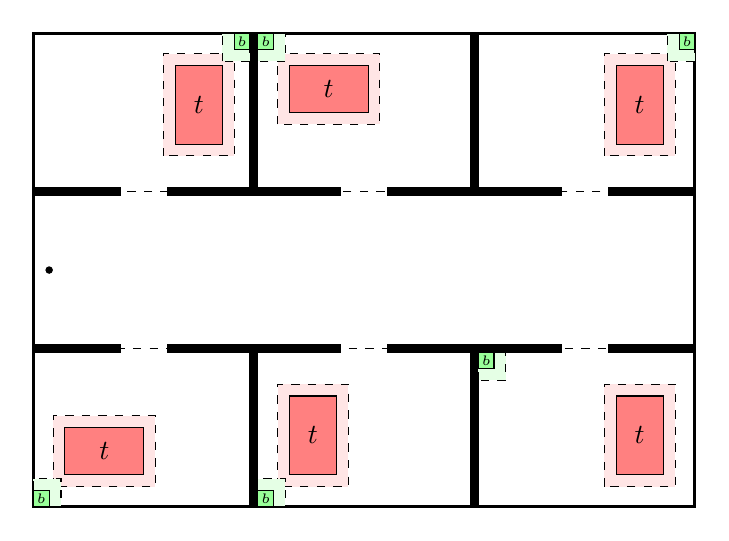
\begin{tikzpicture}
    
        % Boundary
        \draw[very thick, fill = white] (0, 0) rectangle (8.4, 6);
        \draw[dashed] (0,2) -- (8.4,2) -- (8.4, 4) -- (0,4);
        
        % Vertical walls
        \filldraw (2.75, 0) rectangle (2.85, 2.05);
        \filldraw (2.75, 3.95) rectangle (2.85, 6);
        \filldraw (5.55, 0) rectangle (5.65, 2.05);
        \filldraw (5.55, 3.95) rectangle (5.65, 6);
        
        % Horizontal walls
        \filldraw (0, 1.95) rectangle (1.1, 2.05);
    	\filldraw (0, 3.95) rectangle (1.1, 4.05);
        \filldraw (1.7, 1.95) rectangle (3.9, 2.05);
    	\filldraw (1.7, 3.95) rectangle (3.9, 4.05);
        \filldraw (4.5, 1.95) rectangle (6.7, 2.05);
    	\filldraw (4.5, 3.95) rectangle (6.7, 4.05);
        \filldraw (7.3, 1.95) rectangle (8.4, 2.05);
        \filldraw (7.3, 3.95) rectangle (8.4, 4.05);
        
    	% Table label lines
    	\filldraw[dashed, fill = red!10!white] (0.25,0.25) rectangle (1.55,1.15); % r1
    	\filldraw[dashed, fill = red!10!white] (1.65,4.45) rectangle (2.55,5.75); %r2
    	\filldraw[dashed, fill = red!10!white] (3.1,0.25) rectangle (4,1.55); % r3
    	\filldraw[dashed, fill = red!10!white] (3.1,4.85) rectangle (4.4,5.75); %r4
    	\filldraw[dashed, fill = red!10!white] (7.25,0.25) rectangle (8.15,1.55); % r5
    	\filldraw[dashed, fill = red!10!white] (7.25,4.45) rectangle (8.15,5.75); %r6
    	
    	% Bin label lines
    	\filldraw[dashed, fill = green!10!white] (0,0) rectangle (0.35,0.35); % r1
    	\filldraw[dashed, fill = green!10!white] (2.4,5.65) rectangle (2.75,6); % r2
    	\filldraw[dashed, fill = green!10!white] (2.85,0) rectangle (3.2,0.35); % r3
    	\filldraw[dashed, fill = green!10!white] (2.85,5.65) rectangle (3.2,6); % r4
    	\filldraw[dashed, fill = green!10!white] (5.65,1.6) rectangle (6,1.95); % r5
    	\filldraw[dashed, fill = green!10!white] (8.05,5.65) rectangle (8.4,6); % r6
    	
    	% Bins
    	\filldraw[fill = green!40!white] (0, 0) rectangle (0.2, 0.2) node[midway] {\tiny $b$}; % r1
    	\filldraw[fill = green!40!white] (2.55, 5.8) rectangle (2.75, 6) node[midway] {\tiny $b$}; % r2
    	\filldraw[fill = green!40!white] (2.85, 0) rectangle (3.05, 0.2) node[midway] {\tiny $b$}; % r3
    	\filldraw[fill = green!40!white] (2.85, 5.8) rectangle (3.05, 6) node[midway] {\tiny $b$}; % r4
    	\filldraw[fill = green!40!white] (5.65, 1.75) rectangle (5.85, 1.95) node[midway] {\tiny $b$}; % r5
    	\filldraw[fill = green!40!white] (8.2, 5.8) rectangle (8.4, 6) node[midway] {\tiny $b$}; % r6
    	
    	% Tables
    	\filldraw[fill = red!50!white] (0.4, 0.4) rectangle (1.4, 1) node[midway] {$t$}; % r1
    	\filldraw[fill = red!50!white] (1.8, 4.6) rectangle (2.4, 5.6) node[midway] {$t$}; % r2
    	\filldraw[fill = red!50!white] (3.25, 0.4) rectangle (3.85, 1.4) node[midway] {$t$}; % r3
    	\filldraw[fill = red!50!white] (3.25, 5) rectangle (4.25, 5.6) node[midway] {$t$}; % r4
    	\filldraw[fill = red!50!white] (7.4, 0.4) rectangle (8.0, 1.4) node[midway] {$t$}; % r5
    	\filldraw[fill = red!50!white] (7.4, 4.6) rectangle (8.0, 5.6) node[midway] {$t$}; % r6
    	
    	\filldraw[black] (0.2, 3) circle (0.4mm);
    \end{tikzpicture}
    }
    \caption{Example of an office-like environment used in the case study. Black solid lines represent walls. There are six rooms, each labeled with one atomic proposition $r_i$, for $i \in [1,6]$, and a hallway labeled $h$. Each room contains a table (red) and a bin (green), labeled $t$ and $b$, respectively. The labels of tables and bins hold true within the corresponding dashed and shaded areas surrounding it. The initial position of the robot is marked with a black dot on the left side of the hallway.}
    \label{fig:example}
\end{figure}



The scLTL specification is inspired by a realistic scenario, common in every office environment: reach a wastebin in the office rooms. We translate such a specification to the following scLTL formula:
\begin{equation}
    \varphi = \F(r_1 \wedge b) \wedge \F (r_2 \wedge b)\wedge \dots \F (r_6 \wedge b) \label{eq: spec}
\end{equation}
%
Note that such a specification does not impose any ordering of events.

For information gain, we use the following functions in our simulations
% Regarding the calculation of the information gains $\mathrm{IG_{map}}, \mathrm{IG_{bias}}$, given a \emph{map} frontier $m$, a \emph{bias} frontier $x_s$, and the current position $p$ of the robot, we use the following equations in our simulations:
%
\begin{align}
    \mathrm{IG_{map}}(m, p) &= \frac{\mathrm{size}_m}{d_{m, p}} \\
    \mathrm{IG_{bias}}(x_s, p) &= \frac{a}{r^{b}_{x_s} \, d_{x_s, p}}
\end{align} % this was that way so it would occupy less space
%
where $\mathrm{size}_m$ is the size of frontier $m$, $d_{m, p}$ and $d_{x_s, p}$ are the length of the shortest path between $p$ and $m$ and $x_s$, respectively, $a,b > 0$ are  user-defined parameters, and $r_{x_s}$ is the rank of $x_s$. Adjusting $a,b$ is intuitive: i) suppose $m$ and $x_s$ are equidistant from $p$; ii) fix $r_{x_s}$ to 1 and choose $a$ to reflect how a \emph{bias} frontier compares to a \emph{map} frontier; iii) now suppose $x_{s,1}, x_{s,2}$ equidistant from $p$, such that $r_{x_{s,1}}~=~1$ and $r_{x_{s,2}} = 2$; iv) choose $b$ as to reflect how the importance of \emph{bias} frontier decays with its rank (e.g. linearly, quadratic). For our case study, we chose $a=100$ and $b=2$.

\begin{table*}%[th]
    \centering
    \caption{Mean and standard deviation of the total trajectory length to satisfy the scLTL mission \eqref{eq: spec}, along with total runtime and RRG size. The results were drawn from simulating each approach 3 times in each of the 100 randomly-generated environments.}\label{tab:my_label2}
    \setlength{\tabcolsep}{3pt}
    \footnotesize
    \begin{tabular}{l c c c | c c c }
        \toprule
        \textbf{} & \multicolumn{3}{c}{\textbf{See-through Desks}} & \multicolumn{3}{c}{\textbf{Opaque Desks}} \\
        \cmidrule(lr{.75em}){2-4} \cmidrule(l{.75em}r){5-7}
		&\textbf{\sep}&\textbf{\tog}&\textbf{\bia}&\textbf{\sep}&\textbf{\tog}&\textbf{\bia}\\
		\midrule
		\textbf{Total length}     & 77.3 (7.5) & 56.6 (8.0) & 29.4 (5.0) & 79.1 (7.1) & 62.9 (16.5) & 32.3 (11.8) \\
		%%
		\multicolumn{1}{l}{Exploration length}  & 57.1 (3.2) & 37.5 (7.1) & 28.0 (4.9) & 57.8 (4.9) & 44.4 (16.6) & 31.3 (12.1) \\
		%\hline
		\multicolumn{1}{l}{Remaining plan l.} & 20.2 (7.0) & 19.1 (3.6) & 1.3 (1.8) & 21.3 (5.1) & 18.5 (3.4) & 1.1 (1.8)\\
		%%
		\textbf{Total Time}       & 7.8 (2.0) & 6.4 (2.3) & 7.3 (1.9) & 9.6 (2.5) & 8.3 (3.2) & 9.1 (2.4)\\
		%%
		\textbf{RRG size}         & 1931.2 (460.9) & 1938.6 (559.5) & 1793.6 (312.1) & 2313.8 (550.9) & 1868.7 (498.2) & 1901.4 (301.2)\\
		\bottomrule
    \end{tabular}
\end{table*}

\begin{figure*}
    \centering
    \subfloat[\label{fig:tog0}]{\includegraphics[width = 0.33\linewidth]{figures/tog_firstMove.png}}
    \subfloat[\label{fig:tog1}]{\includegraphics[width = 0.33\linewidth]{figures/tog_room.png}}
    \subfloat[\label{fig:tog2}]{\includegraphics[width = 0.33\linewidth]{figures/tog_final.png}} \\
    \subfloat[\label{fig:sep0}]{\includegraphics[width = 0.33\linewidth]{figures/sep_bin.png}}
    \subfloat[\label{fig:sep1}]{\includegraphics[width = 0.33\linewidth]{figures/sep_room.png}}
    \subfloat[\label{fig:sep2}]{\includegraphics[width = 0.33\linewidth]{figures/sep_final.png}}
    \caption{Snapshots of the robot navigating the office environment in the attempt to satisfy the scLTL mission \eqref{eq: spec} with two different approaches. The yellow semi-circle in (a) corresponds to the robot's sensing radius. The top-row figures (a-c) display the trajectory (green) when using the approach proposed by us (SAG-RRG), where exploration and planning are done together; the bottom-row figures (d-f) show the case where the robot first explores the environment, and only then it plans a path that satisfies the mission. The RRG graph at the time of the snapshot is shown in blue, and the path that leads to satisfaction of the mission is in red (c,f).}
    \label{fig:snaps}
\end{figure*}

The results are presented in Table~\ref{tab:my_label2} for 100 randomly-generated environments. 
The solution presented in this paper can be seen as an approach that performs exploration of the environment and planning to satisfy the scLTL mission concurrently, without or with bias in building the RRG tree (`Simultaneous' and `Simult. biased' columns in Table~\ref{tab:my_label2}). We compare this integrated solution to the trivial sequential approach (`Explore, then plan' column in Table~\ref{tab:my_label2}), which consists of first exploring the whole environment, and then planning a trajectory that satisfies the mission. Lastly, in a more technical variant regarding the sensing capabilities of the robot, we analyse two cases, one where the robot can ``see through'' the desks (e.g., a flying robot), and another where they are considered to be Opaque. A few snapshots of the robot trajectory are shown in Fig.~\ref{fig:snaps}. Each approach is run three times in each of the 100 environments, totalling 1800 runs of the experiment.


The rows in Table~\ref{tab:my_label2} display the length (`Total length') of the trajectory traversed by the robot, from its initial state (common to all cases) until mission satisfaction, as well as the total computation time (`Total time') and number of nodes in the RRG graph (`RRG size'). Additionally, we also display the `Exploration length' which, for the sequential approach, represents the length of the trajectory traversed only during the exploration phase, while for our approach it represents the length traversed until the system realises that a trajectory that satisfies the mission already exists. `Remaining plan l.' is the length of the remaining trajectory that needs to be followed in order to satisfy the desired specification at the moment when exploration phase ends in the `Explore, then plan' case, or the moment when the trajectory is found in the `Simultaneous' and ´Simult. biased' cases. In Table~\ref{tab:my_label2} we see that having ``see-through'' desks makes the performance (both total length and time) slightly better in all the cases, which is to be expected as there are not as many occlusions in the map as with ``opaque'' desks. 
We also see that exploration and planning together performs better in general and including the bias makes it more than 2.5 times better than the naive approach in terms of the path length.

In the `Explore, then plan' case, the robot's visits to wastebins during the exploration do not count towards the mission satisfaction, in contrast to the `simultaneous unbiased' case. This is one of the reasons the latter performs better, as expected. The `simultaneous biased' version performs a lot better because it was able to visit a lot of wastebins (with the help of biasing) already during the exploration.

%There are two approaches to solve the problem (i) first do pure exploration then do planning in a known environment, explore and plan together, (ii) trying to satisfy the property while exploring. There can be two variants of both the approaches, with biasing and without biasing. We compare all 4 algorithms on the office like environment described earlier. We ran all 4 variants 100 times and present the average results in table \ref{tab:resultsseethrough} along with the standard deviation.

%Let us start by evaluating the case where the environment is completely known \emph{a priori}. Even though it might seem that the average time taken to find a solution when using the proposed approach is not a large improvement over the unbiased version, we highlight here the difference on the number of iterations taken until a solution was found. In the unbiased version, the algorithm spends a long time expanding the RRG graph randomly, creating a large graph that leads to unnecessary locations in the environment. On the other hand, our algorithm does not grow such a large graph (a third the size of the unbiased version), but invests time learning about the environment and biasing its search towards relevant regions.

%Such a difference becomes even more apparent if the environment is completely unknown \emph{a priori}. Even though both biased and unbiased versions are using the same underlying approach to explore the environment (frontier exploration \cite{yamauchi1997frontier}), our algorithm performs on average eight times faster, with an eighth of the nodes required by the unbiased version to find a satisfying path.







\section{CONCLUSIONS AND FUTURE WORK}\label{sec:conclusion}
We presented an online sampling-based algorithm capable of finding a trajectory in an \emph{a priori} unknown environment that satisfies an scLTL specification. We enrich the RRG algorithm with functions that attempt to learn possible relations between labels of the environment and use such relations for biasing the search for a satisfying trajectory. The resulting paths are significantly shorter than in straightforward sequential exploration followed by planning in a known space.

A few topics to be considered for future work include extending the approach to consider probabilistic relationships in the semantic abstraction of the system, as well as the extension to multi-agent systems.


%\addtolength{\textheight}{-12cm}   % This command serves to balance the column lengths
                                  % on the last page of the document manually. It shortens
                                  % the textheight of the last page by a suitable amount.
                                  % This command does not take effect until the next page
                                  % so it should come on the page before the last. Make
                                  % sure that you do not shorten the textheight too much.

%%%%%%%%%%%%%%%%%%%%%%%%%%%%%%%%%%%%%%%%%%%%%%%%%%%%%%%%%%%%%%%%%%%%%%%%%%%%%%%%



%%%%%%%%%%%%%%%%%%%%%%%%%%%%%%%%%%%%%%%%%%%%%%%%%%%%%%%%%%%%%%%%%%%%%%%%%%%%%%%%



%%%%%%%%%%%%%%%%%%%%%%%%%%%%%%%%%%%%%%%%%%%%%%%%%%%%%%%%%%%%%%%%%%%%%%%%%%%%%%%%
%\section*{APPENDIX}

%\section*{ACKNOWLEDGMENT}




%%%%%%%%%%%%%%%%%%%%%%%%%%%%%%%%%%%%%%%%%%%%%%%%%%%%%%%%%%%%%%%%%%%%%%%%%%%%%%%%
% IROS:
%\bibliographystyle{IEEEtran}
% RSS:
\bibliographystyle{plainnat}

\bibliography{literature}

\end{document}
